\documentclass[]{article}


\author{Silvio Gregorini}
\title{}
\date{2019}

% Ask if it's possible to use a two column layout
\usepackage[utf8]{inputenc}
\usepackage{csquotes}
\usepackage[english]{babel}
\usepackage{xcolor}
\usepackage{hyperref}
\usepackage{graphicx}
\usepackage{pdflscape}
\usepackage{appendix}
%\usepackage[style=authoryear]{biblatex}
%\addbibresource{bibliography.bib}

\hypersetup{
  colorlinks   = true, %Colours links instead of ugly boxes
  urlcolor     = black, %Colour for external hyperlinks
  linkcolor    = black, %Colour of internal links
  citecolor   = black %Colour of citations
}

\newcommand{\bibTitle}[1]{\emph{#1}}
\newcommand{\bibYear}[1]{(#1)}
\newcommand{\bibUrl}[1]{\textless#1\textgreater}
\newcommand{\bibUrldate}[1]{[Accessed #1]}

\newcommand{\citeInText}[2]{#1 (#2)}

% Change appearance of numeric labels in citation call-outs
\usepackage{cite}
\renewcommand\citeleft{(}
\renewcommand\citeright{)}

% Change appearance of numeric labels in bibliography 
\makeatletter
\renewcommand{\@biblabel}[1]{}
\makeatother

%\renewcommand{\urlbordercolor}{0} {0} {0}

\begin{document}

%================================================================================
%PUT NUMBERS ON PARAGRAPHS
\begin{titlepage}
    
    \vfill
    \hspace*{-2cm}{\LARGE\textbf{VolcaBoy -- Product Development Plan}}\\[10pt]
    \hspace*{-1cm}{\Large  Assignment 1 - Project Proposal}\\[8pt]
    \hspace*{-1cm}{\large Interfaces and Interactivity - 31419 - AUT - 201820}\\
\vskip12cm
\hspace*{\fill} {\Large Silvio Gregorini}\\[4pt]
\hspace*{\fill} {\large ID: 77203842}\\[4pt]
\hspace*{\fill} {\large 8 November 2019}
    \vfill
    \vfill
    \vfill
\end{titlepage}

\tableofcontents
\pagebreak
\section{Introduction} %DONE

    The aim of this paper is to propose the design and production of an 
    hardware synthesizer, starting from an existing digital sound engine.
    In the sections that follow, it will be explained the background and the rationale 
    behind the project, as well as the initial research undertaken.
    Then, it will be depicted a "blueprint" of the product: the general concept, the 
    architecture of the system -- both hardware and software -- and the production plan 
    will be covered in detail.
    In the last part the evaluation criteria will be set, in order to have a concrete measure
    of the work outcomes.

\section{Background and Motivation}

    This project has been shaped and will be realised keeping as a pivotal point the
    \emph{chiptune} subculture and its principles. As will be discussed in the next paragraphs,
    the product is conceived to be used by people already familiar with the environment and 
    limitations of this musical style. Its purpose is to give users a different and more 
    modern way to interact with a well-known set of sounds and synthesis capabilities.

    \subsection{Pushing the Limits Using Contraints}
        \paragraph{Chiptune} %DONE
        As stated by Collins et al. (2014 )\nocite{COLLINS2014} the term \emph{chiptune} has multiple 
        definitions. Also known as \emph{chip music} or \emph{8-bit music}, it derives from the sound chips that,
         in the first generation of computers and gaming consoles,
         were used to balance the processing power of generating sound effects and music from the
        CPU. In its strictiest meaning, chiptune is used to refer to music created entirely from the original, vintage audio 
        chips. Nevertheless, modifications that do not alter the nature of the sound produced are allowed.\\
        The broadest definition is more related to the aesthetics of the sound, rather then to the source
        generating it. The entire subculture which gravitates around the foundations and features of chip
        music can be called \emph{chiptune} too. Anyway, this paper and the related project will try to stick
        to the strictiest definition of the word, in order to create a product able to maintain the sound fidelity
        of the old processors.

        \paragraph{DMG-001 and trackers} %DONE
        In particular, the following study focuses on the Nintendo DMG-001 from 1989, known with the commercial 
        name of \emph{Game Boy}, which is supposedly one of the most popular tools for the production of chip music.
        From the official datasheet (Nintendo, 2019)\nocite{NINTENDO2019}, this portable console runs on a custom 
        \emph{Sharp LR35902} 8-bit CPU, similar to the \emph{Zilog Z80}\footnote{Popular 8-bit microprocessor widely used 
        from the 1970s to the mid-1980s in desktop and home computers, military applications, synthesizers, arcade machines\ldots} 
        and has four audio channels\footnote{To be precise, as stated in the 8BC Chiptune Wiki (2007)\nocite{8BCCHIPTUNE2007}, 
        the console has a fifth -- and least known -- channel: it is an analogue input channel that allows 
        external synthesis on cartridge to be mixed with the sound generated by the other channels. No cartridges 
        are known to use this channel and its functionality, though.}:\\
       
        \def\arraystretch{1.2}
        \begin{table}[h!]
            \begin{tabular}{l l l}
                \hline
                \textbf{Channel} & \textbf{Type} & \textbf{Features}\\
                \hline \\[-6pt]
                1 & Quadrangular\footnotemark & - Volume envelope\\
                    &   &                                                                          - 4-mode pulse width\\
                    &   &                                                                          - Frequency register from C3 upwards\\
                    &   &                                                                          - Frequency envelope\\            
                \hline
                2 & Quadrangular & - Volume envelope\\       
                &   &              - 4-mode pulse width\\
                &   &              - Frequency register from C3 upwards\\
                \hline
                3 & Wave & - User-definable waveforms\\
                &   &      - Bank of 32 samples (4-bit each)\\
                &   &      - Frequency register from C2 upwards\\
                \hline
                4 & Pseudo-random noise & - White and brown noise\\
                \hline \\
            \end{tabular}
            \caption{Sound channels of the Nintendo Game Boy DMG-001.}
        \end{table}
        \footnotetext{Also known as \emph{pulse wave} or \emph{square wave}.}
        
        \nocite{MARQUEZ2014}

        Back in the analog era (i.e. before the first DAWs were created and deployed), the tools to compose and produce music on digital 
        computers and consoles were the \emph{music trackers}. They can be defined as precursors of the modern 
        music production softwares: notes, parameters, effects and other commands, in this type of vertical sequencer, are given
        as letters, numbers or hexadecimal digits into a fixed, time-slotted grid. Fig.\ref{fig:lsdj} shows an
        example of a tracker interface: \emph{Little Sound Dj}, the most popular music editor for 
        Game Boy consoles. The implementation of this tracker, along with other softwares like \emph{nanoloop} 
        and \emph{mGB}, will be considered in the design of the proposed product. \\

        \begin{figure}[h]
            \centering
            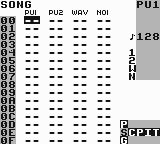
\includegraphics[width=.5\textwidth]{lsdj-song-screen.png}
            \caption{\emph{Song} Screen on the popular LSDJ tracker for Game Boy \cite{KOTLINSKI2007}}
            \label{fig:lsdj}
        \end{figure}


    \subsection{Rationale: Conscious Limitations}
            Despite being one of the cardinal points in the \emph{Chiptune} subculture, the idea of 
            maintaning the limitations given by the hardware is too general and vague, and a distinction is 
            necessary. During the composition and execution of 8-bit music, two main types of constraints can be addressed:

            \begin{itemize}
            \item \textbf{Processing capabilities} -- The true and interesting challenge, i.e. to try to push the 
                    hardware CPU to its limit, creating complex sounds and tracks on a level that was considered 
                    unachievable, given the limited digital resources.
            \item \textbf{User interface} -- Even though someone could disagree with this opinion, from a practical view, limitations in the UI
                    can be considered nothing more than an obstacle in the production process. If we take the DMG-001 as an example, being constrained
                    by a D-pad and four push buttons has nothing to share with the concept of taking out deep and articulated music from a 4.19 MHz CPU with 8 KB of RAM.
            \end{itemize}

            So, it is clear that a limitation in the UI is unnecessary and -- most of the time -- unwanted. For this reasons, the aim 
            behind the proposed product is to renew the link between chiptune musicians and instruments, expanding the interactive capabilities of the Game Boy, 
            without perverting the characteristic soundscape and the core aspects of its composition process.\\
            The product is aimed at whoever wants to use a Nintendo Game Boy as a tool to create music rather than as a videogame console: music producers,
            musicians, beginners and experts will have the chance to interface more easily with the 8-bit music culture, both in 
            composition and live performance contexts.

\section{Project VolcaBoy}
    \subsection{Concept}\label{concept}
            As previously introduced, the core idea behind the product is to create a new and modern interface to mediate between the 
            sound engine and the consumer. The key features which can be outlined from the first design stage are the following, in order of importance:

            \begin{enumerate}
                \item \textbf{Ease of use} -- The main feature of the product. A modern, straightforward interface to interact with the system. The preliminary
                        idea is to create a sequencer-like product, trying to mimic with the hardware what trackers like LSDJ do via software.
                \item \textbf{Portability} -- In order to keep the essence of the Game Boy, which is the most iconic portable console, the product must be small, 
                        easy to carry, and battery powered.
                \item \textbf{Compatibility} -- If possible, the choice is to realise a product able to connect and share data with other digital musical instruments, 
                        to expand the boundaries of chiptune music outside its strictiest definition.
                \item \textbf{Aesthetics} -- Although not mandatory, appearance is important. Therefore, attention must also be paid 
                        to the aesthetic part of the design, rather than focusing only on functionality.
            \end{enumerate}
            
            As it could be guessed by the above list, during the initial design stage it became more and more obviuos the similarity of this potential product with a 
            type of musical tools already on the market: the \emph{Korg Volca Series}. On Korg website (2019), the volca series is presented as follows: 
            \begin{quote}
                ``This series includes a variety of units such as synthesizers, drum machines, and bass synths that 
                all play a specialized role in your performance or studio setup. Users can perform with multiple units using the tempo sync 
                included on all volcas. The compact design of the Korg volca series 
                is packed with limitless possibilities.'' \cite{KORG2019}
            \end{quote}

            Therefore, the decision was taken to use this series of synthesizers as a principal inspiration for what 
            concerns dimensions, functionalities and overall appearance of the final product. To better understand the 
            components and the layout of the above mentioned synthesizers, in Appendix A can be found the assembly sketch of a Korg Volca Bass. %APPENDIX A

            \begin{figure}[h]
                \centering
                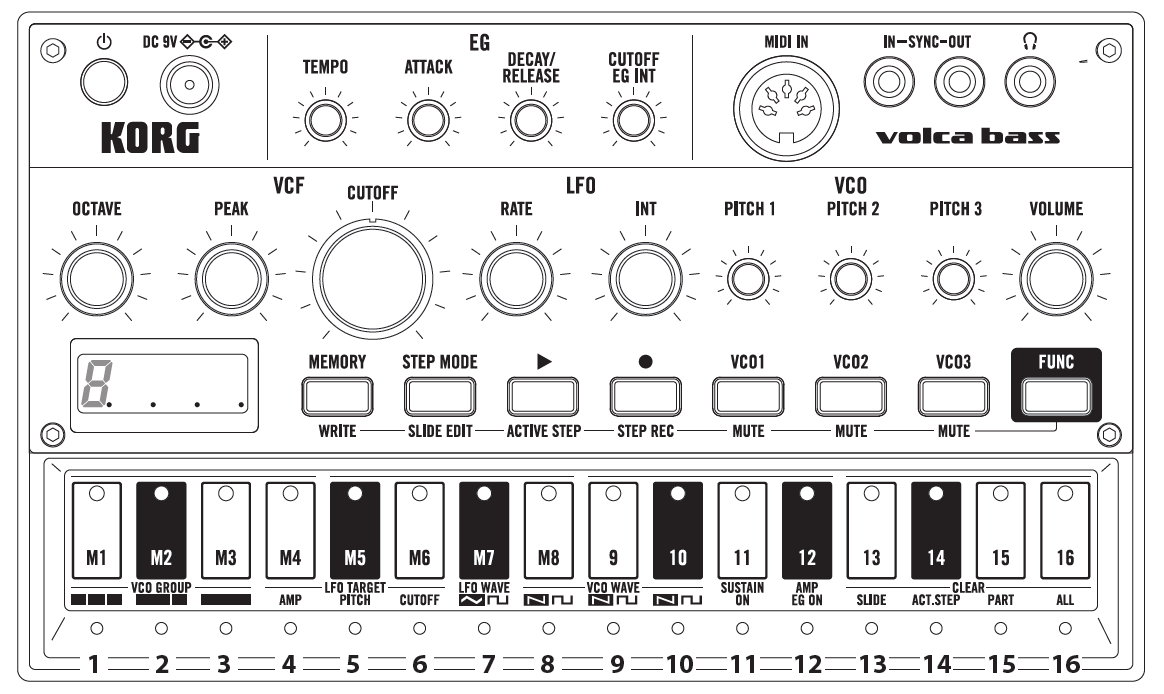
\includegraphics[width=\textwidth]{korg-volca-bass.png}
                \caption{Front view of a \emph{Korg Volca Bass} \cite{KORG2013}.}
                \label{fig:volcabass}
                
            \end{figure}

    \subsection{System Architecture}
            In the following section the overall architecture of the product will be explained. Since the design and 
            production process is not conventional -- i.e. the product is not to be manufactured from scratch, like in a 
            standard, professional context --, this part of the paper is separated in three main subsections, in order to 
            follow the steps of the manufacturing process: hardware, DMG-001 modifications and software.
            
        \subsubsection{Hardware}
            \paragraph{Controls}
            In order to translate a tracker's GUI into a physical interface, the structure of a step sequencer turned out to be the most suitable. Hence,
            the product would have a grid of push buttons to map each channel and beat of the DMG-001, a digital rotary encoder to choose the note for a selected beat
            and an analog potentiometer to control the level of the master volume\footnote{This distinction between volume and note potentiometer is made necessary by how the signals will 
            be routed: the master volume will be hijacked directly from the console's motherboard, so it will be a continuous, analog signal. On the other hand, the note selection
            will be made on the Arduino embedded software, and it will be a discrete, digital signal -- this topic will be expanded in \ref{software}.}.

            Furthermore, considering that, in a professional environment, the entire project depicted in this paper could be associated with the prototyping stages of a commercial product
            the decision was made to keep the original controls of the console for debugging purposes. 
            But, while proceeding with the preliminary blueprint, a problem related to this design emerged: sticking blindly to the step sequencer idea would mean to have a grid of 4 x 16 buttons
            \footnote{Four rows for the console channels and sixteen columns for the beats because, working on hexadecimal values, most of the trackers 
            had this time subdivision.}, which is an issue when considering the portability of the system.

            \paragraph{User Interface}\label{userinterface}
            To address the problem, it has been chosen to reduce the number of physical controls and implement a digital UI with minimal features, to 
            balance between the \emph{ease of use} and the \emph{portability} of the product. Therefore, the push buttons grid will be reduced to 
            4 x 8 and splitted in two pairs of rows: the first will handle two channels from beat 1 to 8, the second will handle the same two channels
            from beat 9 to 16. Then, the channels will be grouped in \emph{banks}:
            \begin{itemize}
                \item \textbf{Bank A} -- Channel 1 and 2;
                \item \textbf{Bank B} -- Channel 3 and 4;
            \end{itemize}
            Concretely, the grid is to be built following the electric schematic of a \emph{keyboard matrix}\footnote{Refer to Trybus, M. (2013)\nocite{TRYBUS2013} for a general explaination of this concept.}, and two additional buttons will be added 
            to select which bank to open in the sequencer grid. Finally, a dedicated LCD screen will show which bank, parameter, note or control is being tweaked. Figure \ref{frontview} shows how, potentially, the UI could appear, while in Appendix B can be 
            found a complete preliminary design of the product, which has been modeled in SolidWorks and then exported in a standard orthogonal projection format.             % APPENDIX B
            
            \begin{figure}[h]
                \centering
                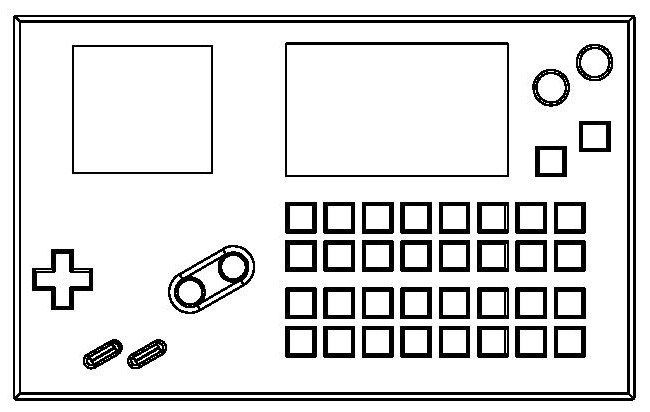
\includegraphics{volca-boy-draw-page-001-front-view.jpg}
                \caption{Front view of the first blueprint of the product.}
                \label{frontview}
            \end{figure}
            
        
        \subsubsection{DMG-001 Mods}\label{mods}
            As anticipated, an important part of this project involves the modification of the Game Boy to modernize its structure and implement additional features.
            Luckily, well documented work has been made by the community in previous years, so the design process in this section can be significantly reduced
            taking advantage of the available online resources. The only obstacle here will be to find the most convenient and efficient way to merge together the
            single mods. Obviously, all the sources will be properly referenced and quoted throughout the duration of this stage, but at the moment the following tutorials 
            are planned to be used:

            \begin{itemize}
                \item \textbf{Prosound Mod} -- To amplificate and clean the sound coming out from the console and to add audio sockets more suitable for a 
                        music production context (e.g. 6.3 mm stereo jack, RCA connectors\dots). For this mod the tutorials from 8bitjunkie (2014)\nocite{8BITJUNKIE2014} 
                        and Benn Venn (2018)\nocite{BENNVENN2018} will be followed.
                \item \textbf{ArduinoBoy} -- The most important mod to be done, it will give the console the ability to send and receive midi messages and therefore 
                        allow the Game Boy to communicate with the controls described above. This step will require an Arduino board and some electronics, but the 
                        documentation provided by trash80 (2017)\nocite{TRASH802017} is detailed and exhaustive.
                \item \textbf{Screen Backlight and Bivert} -- This is only an aesthetic mod, to enhance the contrast and the readibility of the original screen. 
                        It is functionally useless, since all the parameters will be shown on the second screen (see \ref{userinterface}) but, since the appearance of 
                        the finished product matters as well, it will be taken into account. Tutorials from RetroRepairs (2019)\nocite{RETROREPAIRS2019} and This Does Not Compute (2016)\nocite{THISDOESNOTCOMPUTE2016} will be used. 
                \item \textbf{Rechargeable Battery Mod} -- Another key point of the proposed product will be the portability. This modification isn't straightforward 
                        like the others, because the console isn't the only component that needs to be powered, so a deeper analysis is required to design a solution for the 
                        specific case.
            \end{itemize}

        In Appendix C is depicted a comprehensive part list for both the hardware construction and the console modifications.      %_____________________________________________PART LIST     % APPENDIX C 

        \subsubsection{Embedded Software}\label{software}
        At the moment, the product is planned to contain two Arduino boards, so a necessary distinction has to be made: in this paper, for ``embedded software'' is meant only the code 
        which will be written and deployed from scratch. Vice versa, the code made by third-party developers (e.g. the software running on the Arduino board that will manage 
        the stream of MIDI messages) has been covered in \ref{mods}. That said, the embedded software will run on an Arduino Nano 33 BLE and the following features are to be added:\\

        \begin{table}[h!]
            \centering
            \begin{tabular}{|l|l|}
                \hline
                \textbf{Feature} & \textbf{Type}\\
                \hline
                Push buttons grid mapping & Back-end\\
                \hline
                Note rotary encoder mapping & Back-end\\
                \hline
                Conversion from UI (i.e. beat/note selected) to MIDI & Back-end\\
                \hline
                Tempo & Back-end\\
                \hline
                RGB LED mapping & Front-end\\
                \hline
                GUI & Front-end\\
                \hline
            \end{tabular}
            \caption{Key features of the embedded software.}
        \end{table}

        To conclude and summarise this section, in Figure \ref{umldiagram} a schematic of the system architecture can be found.
        The scheme mainly follows the rules to deploy a Unified Modeling Language (UML) \emph{Implementation Diagram} \cite{STEVENS2006}.

        \begin{figure}[h]
            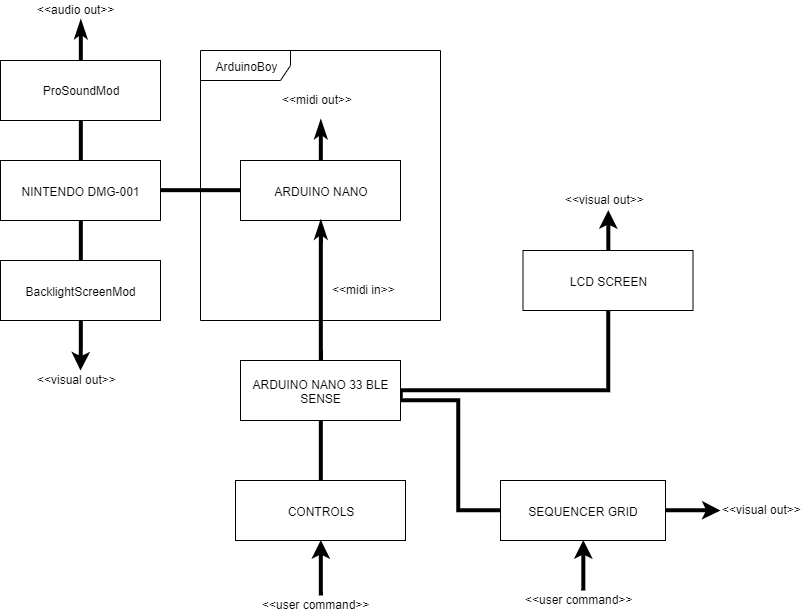
\includegraphics[width=\linewidth]{implementation-diagram.png}
                \caption{UML-style implementation diagram of the system.}
                \label{umldiagram}
            \end{figure} 
        
        \subsection{Production}
            \paragraph{Resources}
            Most of the literature resources that are planned to be used during the production stage are listed in the References section of this paper and
            in the appendices. About the production resources, a \emph{DIY} approach has been chosen for the project, being at once the most cost effective 
            and the most rewarding in terms of knowledge and practical experience. In addition to programming most of the software from scratch, programs like SolidWorks,
            PSpice, Fritzing, Simplify3D will be used to design and simulate the behavior of the system. During the procution stage, tools such as 
            soldering irons, 3D printers and dremels will be employed in the construction of the hardware, consisting of the electrical circuitry and the external enclosure.
            

            \paragraph{Schedule}
            Given the size and complexity of the project, a well organized timescale is mandatory. For the definition of the various stage,
            inspiration was taken by the work of Cunningham (2018)\nocite{CUNNINGHAM2018} and Nandakumar (2018)\nocite{NANDAKUMAR2018}. The idea is to embrace
            a typical electronic product development cycle, so the entire process will be splitted into four categories listed in Table \ref{stages-table}. 
            The detailed version of the timescale -- made using the online project planning tool \emph{TeamGantt} -- can be found in Appendix D. %_________________________ ADD TIMESCALE APPENDIX       % APPENDIX D

            \begin{table}[h!]
                \centering
                \begin{tabular}{|l|l|}
                    \hline
                    \textbf{Stage} & \textbf{Time Period}\\
                    \hline
                    Planning & 30/09 -- 24/11\\
                    \hline
                    Embedded Software & 28/10 -- 15/12\\
                    \hline
                    Hardware & 11/11 -- 05/01\\
                    \hline
                    Production & 08/11 -- 10/01\\ 
                    \hline

                \end{tabular}
                \caption{Product development stages.}\label{stages-table}
            \end{table}


            \paragraph{Health and Safety} %_________________________ ADD RISK ASSESSMENT APPENDIX       % APPENDIX E
            For what concerns the health and safety, in a broad process such as the one considered it is difficult to predict each potential risk and issue,
            since the production line is prone to changes and other manufacturing tools could be employed in the development. However, a risk assessment
            table has been drafted and can be found in Appendix G, with the principal potential risks at the moment.
   
    
        \section{Conclusions}
            To conclude, in this section are listed and discussed the criteria to evaluate the outcomes of the proposed project.

            \paragraph{Minimum Viable Product}
            First, to evaluate the final result of this production process, the Minimum Viable Product has to be defined. In this case, since the primary aim
            of the project is to create a new way for a chiptune producer to interact with a Game Boy, the MVP must show, at least, a different user interface 
            provided with MIDI functionality.

            \paragraph{Evaluation Criteria}
            From this point, the product will be evaluated according to the key features listed in Section \ref{concept}. For example, on a scale from
            1 to 5, the outcome could be assessed as follow:

            \begin{itemize}
                \item[-] \textbf{1/5} -- The product fails to satisfy the features defined in the MVP, a non-working prototype has been made and no documentation
                            has been created;
                \item[-] \textbf{2/5} -- The product satisfies the MVP definition, although the prototype works only under specific conditions and the documentation is 
                            vague and inconsistent;
                \item[-] \textbf{3/5} -- The product adds functionalities to the MVP definition, the prototype works in most testing conditions and basic documentation has been 
                            provided; 
                \item[-] \textbf{4/5} -- The product shows most of the functionalities blueprinted during the design stage, the prototype is fully functional and basic documentation
                            has been provided; 
                \item[-] \textbf{5/5} -- The product is exactly as described during the design stage, the prototype is fully functional and aesthetically appealing, 
                            exhaustive and detailed documentation has been provided. 
                      
            \end{itemize}
        
            Finally, in Appendix F there is a 3D render that simulates how the product could potentially appear if the design and production process proceed as planned.
            
            \pagebreak
            
%=================================================%
%       REMEMBER TO SORT THE BIBLIOGRAPHY
%=================================================%

\begin{thebibliography}{99}

    \bibitem[Collins et al., 2014]{COLLINS2014}
    Collins, K. and Kapralos, B. and Tessler, H. and Paul, J. L.
    \bibYear{2014}
    \bibTitle{The Oxford Handbook of Interactive Audio.}
    USA: Oxford University Press.

    
    \bibitem[Marquez, 2014]{MARQUEZ2014}
    Marquez, I.
    \bibYear{2014}
    Playing new music with old games: The chiptune subculture.
    \bibTitle{G| A| M| E Games as Art, Media, Entertainment}
    [Online], 1 (3), pp. 67-79. Available from: 
    \bibUrl{\url{http://www.gamejournal.it/wp-content/uploads/2014/04/GAME_3_Subcultures_Journal_Marquez.pdf}}
    \bibUrldate{20 October 2019}.


    \bibitem[Nintendo, 2019]{NINTENDO2019}
    Nintendo
    \bibYear{2019}
    \bibTitle{Game Boy, Game Boy Color, Game Boy Pocket Technical Data}
    [Support page] [Online] Available from: 
    \bibUrl{\url{https://www.nintendo.co.uk/Support/Game-Boy-Pocket-Color/Product-information/Technical-data/Technical-data-619585.html}}
    \bibUrldate{20 October 2019}.

\end{thebibliography}



        \begin{appendices}
            \appendix
            \begin{landscape}
                \begin{figure}[h!]
                \textbf{\appendixname{ A}}\\ %VOLCA ASSEMBLY SKETCH
                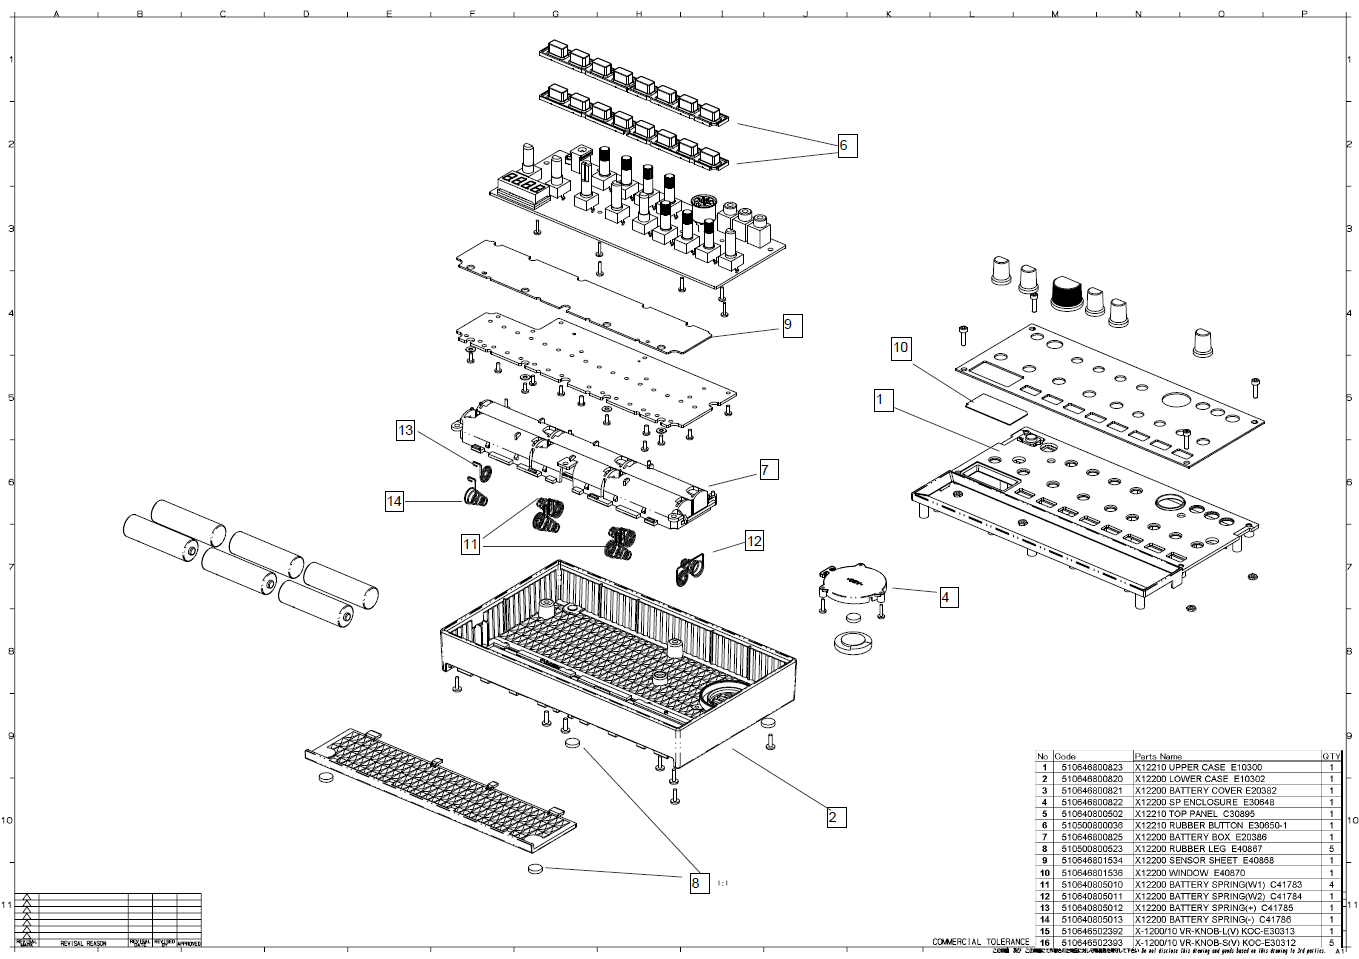
\includegraphics[width=\linewidth]{korg-volca-bass-assembly-sketch.png}
                    \caption{Korg Volca Bass assembly sketch \cite{KORG2013}.}
                \end{figure}
            \end{landscape}
            \pagebreak
            
            \appendix
            \begin{figure}[h]
                \vspace*{-1cm}
                \textbf{\appendixname{ B}}\\   %UI SCHEME
                \hspace*{-1cm}
                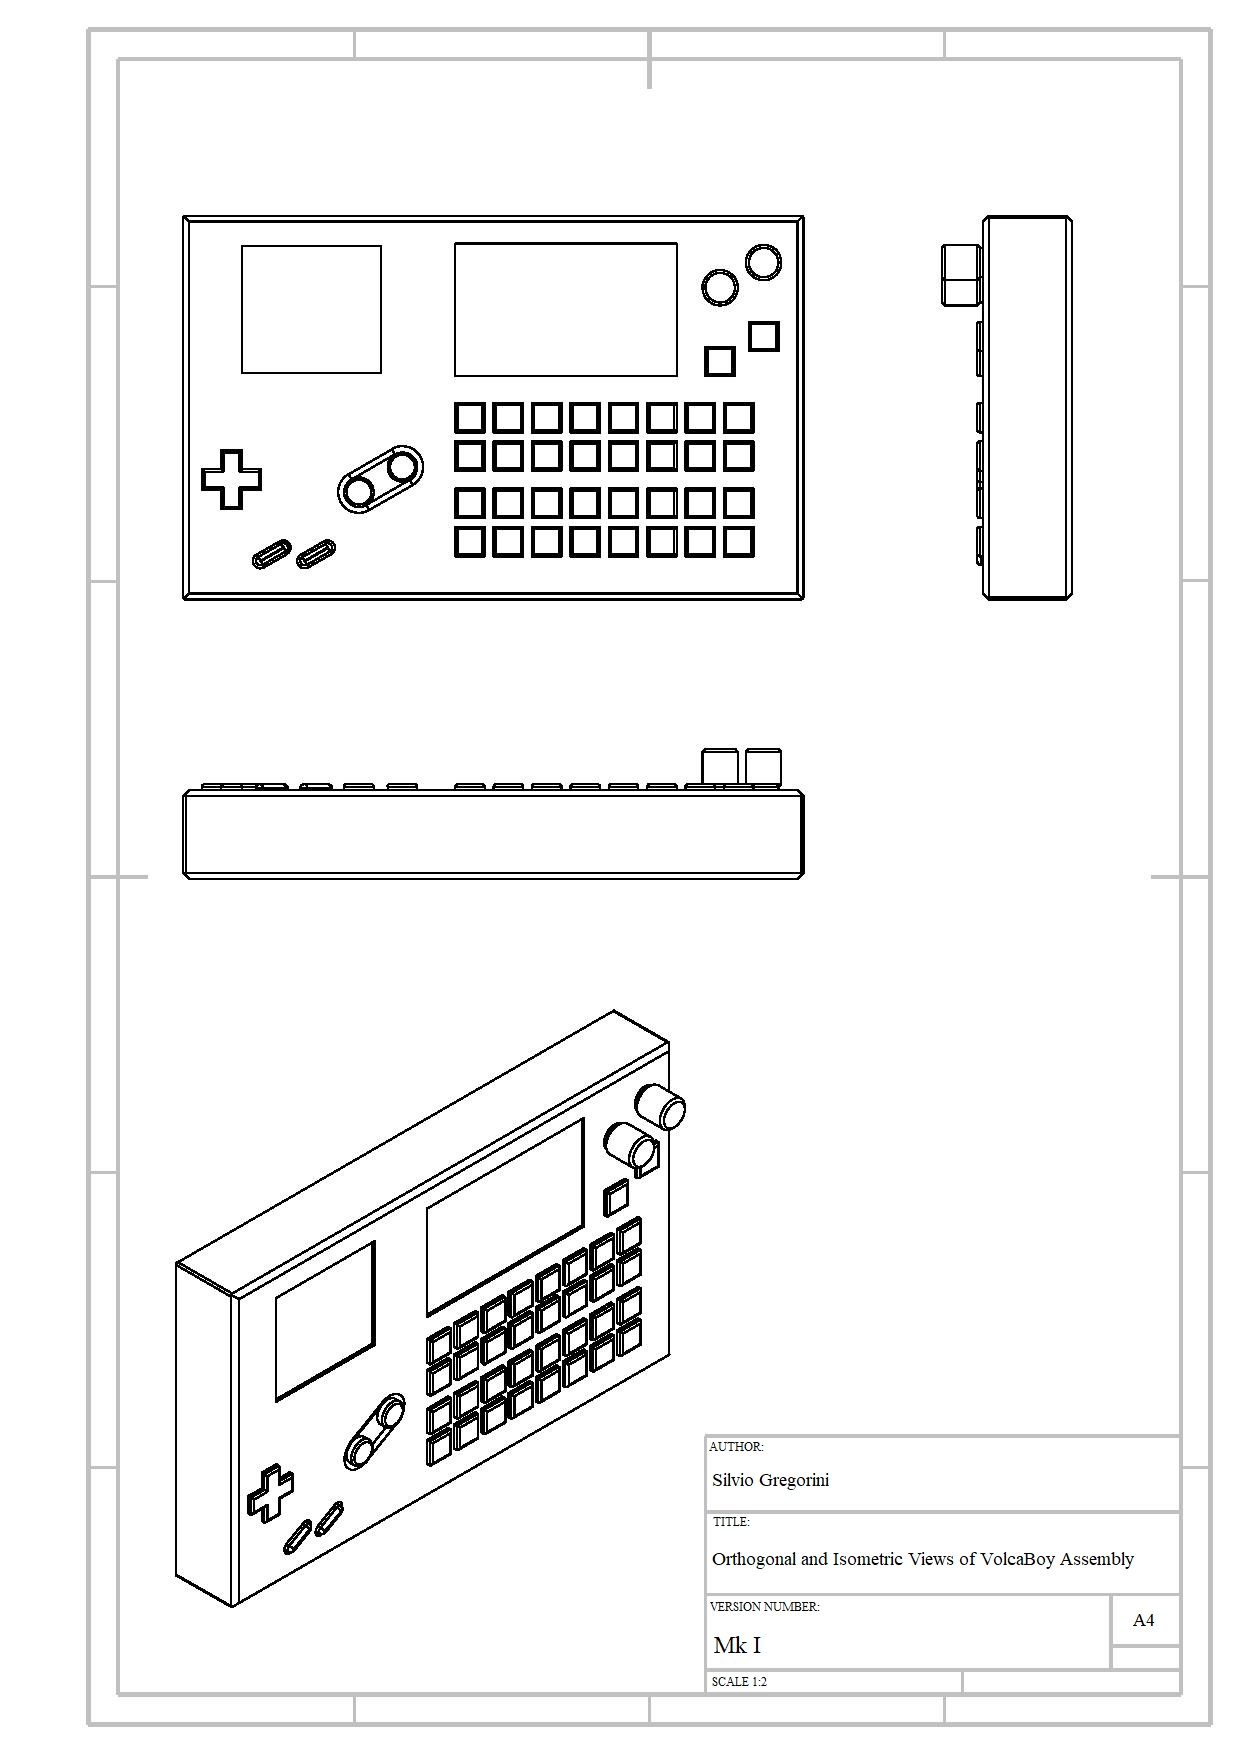
\includegraphics[width=1.1\textwidth]{volca-boy-draw-page-001.jpg}
                    \caption{Orthogonal projectijon and isometric view of a preliminary version of the product, modeled and exported SolidWorks.}
                \end{figure}
\pagebreak

            \appendix
            \begin{table}[h]
                \textbf{\appendixname{ C}}\\  %PART LIST
                
                \centering
                \begin{tabular}{|lcl|} % Sequencer
                    \hline
                    \textbf{Part} & \textbf{Qt.} & \textbf{Link}\\
                    \hline 
                    Arduino Nano 33 BLE Sense & 1 &\url{https://bit.ly/2Q0qRxJ} \\ 
                    2.42" OLED display & 1 & \url{https://amzn.to/2NPwWKy}   \\
                    %Front-lit LED strips & 1 & \url{https://www.sparkfun.com/products/14730}   \\
                    Side-lit LED strips & 1 & \url{https://www.sparkfun.com/products/14731}   \\
                    Push button & 34 & \url{https://amzn.to/2WYsJrX}\\
                    EC11 digital rotary encoder & 1 & \url{https://amzn.to/2pSIuEM} \\
                    Single sided proto board & 1 & \url{https://bit.ly/2Q1aSj0}\\
                    1N4148 diodes & 34 & \url{https://bit.ly/34E9x5q} \\
                    \hline
            \end{tabular}
                \caption{Part list for the construction of the grid and the interface.}
                \vspace*{1cm}
            \begin{tabular}{|llcl|} % Screen
             \hline
            \textbf{Mod} &\textbf{Part} & \textbf{Qt.} & \textbf{Link}\\
            \hline 
            \textbf{ProSound} & PAM8403 digital amplifier & 1 & \url{https://bit.ly/32v7qiQ}\\
                    & Potentiometer & 1 & \url{https://bit.ly/32tcyEp}\\
            \hline 
            \textbf{ArduinoBoy} & Arduino Nano & 1 & \url{https://bit.ly/32xrrWa} \\
                            & 6NI38 optocoupler chip & 1  & \url{https://bit.ly/2NwNeJn} \\
                          & 1N914 diode & 1  & \url{https://bit.ly/2WUUXnA}\\
                            & 220 $\Omega$ resistor & 2  & \url{https://bit.ly/2K2EbgZ}\\
                            & 270 $\Omega$ resistor & 1  & \url{https://bit.ly/2pL285Q}\\
                            & 2 $k\Omega$ resistor & 7  & \url{https://bit.ly/2NvEt2n}\\
                            & Push button & 1  & \url{https://amzn.to/2WYsJrX}\\
                            & 5 pin DIN socket & 2  & \url{https://bit.ly/2oZYhBj}\\
                            & DMG-04 game link cable & 1  & \url{https://bit.ly/2Nt72gO}\\
                            & LED & 6  & \url{https://bit.ly/33vGVLK}\\
            \hline
            \textbf{Backlight Screen} & Screen backlight & 1 & \url{https://bit.ly/2qyCHEA} \\
                   & Bivert chip & 1 & \url{https://bit.ly/2qyCHEA} \\
            \hline
            \textbf{Rechargeable Battery} & 2000mah 2S 15~25C Lipo & 1 & \url{https://bit.ly/32teqwV} \\
            & 2-3S AC Compact Charger & 1 & \url{https://bit.ly/36Ge21r} \\
            \hline
            \end{tabular}
            \caption{Part list for the console modification.}
        \end{table}
        

            \appendix
            \begin{landscape}
                \begin{figure}[h!]
                \textbf{\appendixname{ D}}\\ %TIMESCALE
                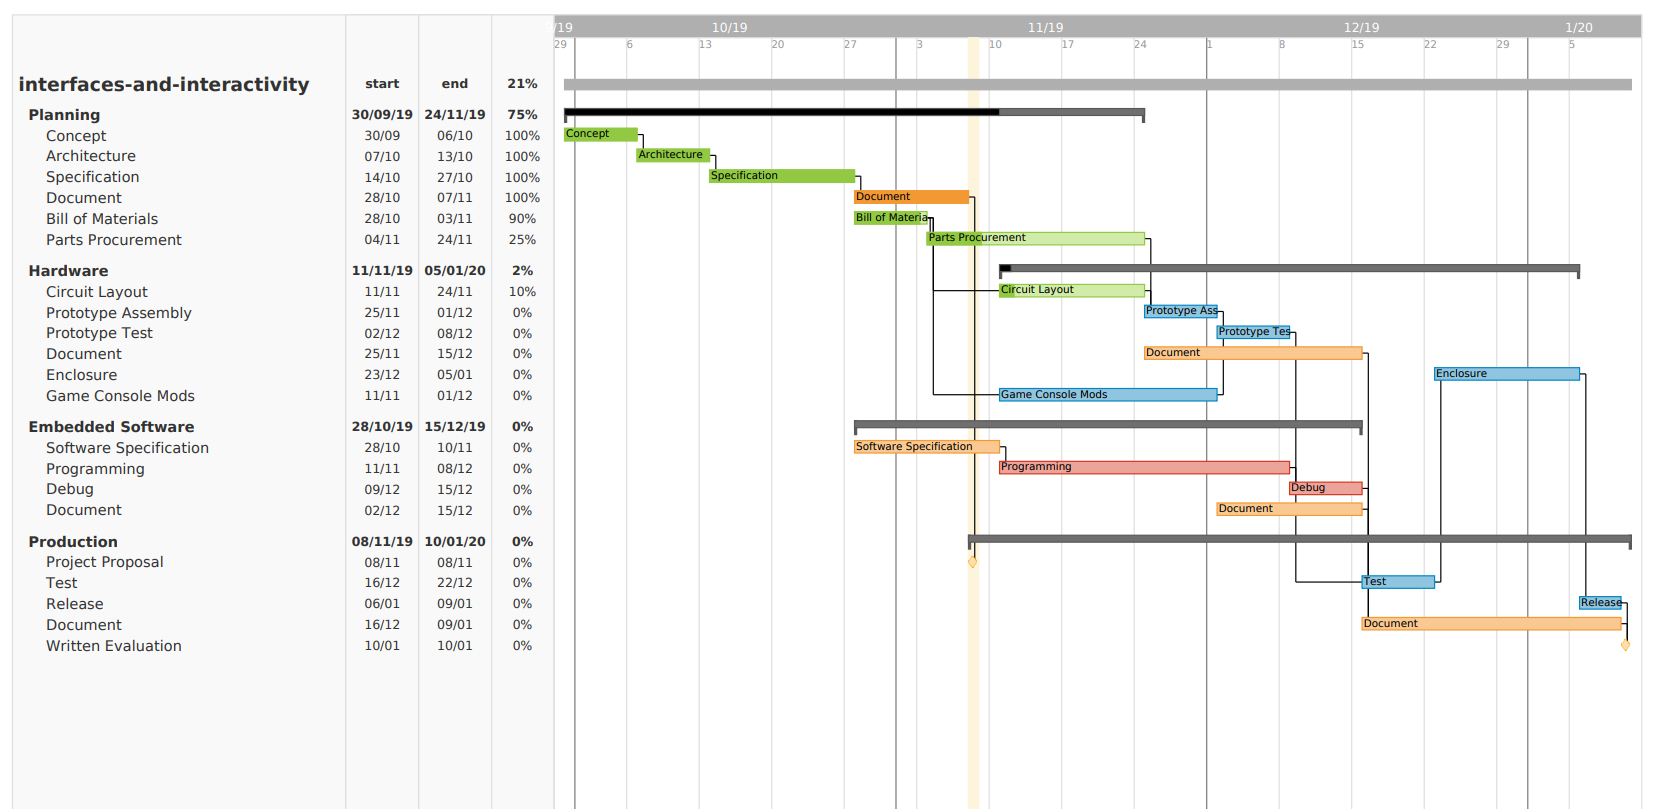
\includegraphics[width=1.1\linewidth]{timescale.png}
                    \caption{Gantt chart showing the product development stages.}
                \end{figure}
            \end{landscape}
       

        \appendix
    \begin{landscape}
        \begin{table}[h!]
            \textbf{\appendixname{ E}}\\ %RISK ASSESSMENT
            
            \centering
            \begin{tabular}{|llll|} \hline
            
                \textbf{Hazards} & \textbf{Risk} & \textbf{Preventative Measures} & \textbf{Remedial Measures} \\
                \hline &&& \\
                Nuisance noise/vibration & Low & - Wear ear protection & - Turn off the operating machine\\
                & & & - In case of injury, seek medical \\ 
                & & & attention\\
                &&&\\
                Hot components & Medium & - Check the 3D printer & - Seek medical attention\\
                & & temperature settings & \\
                & & - Wear protection while soldering & \\
                &&&\\
                Entanglement in moving & Medium & - Step away when the 3D printer & - In case of injury, seek medical \\ 
                machinery & & is moving & attention\\
                &&&\\
                Risk of electric shock & Medium & - Turn off the main power before & - Turn off main power \\
                    &   & touching the electronics & - In case of injury, seek medical  \\
                    &   & - Wear insulated gloves & attention\\
                    &&&\\
                    \hline
            

            \end{tabular} 
            \caption{Risk assessment table.}
        \end{table}

    
    \end{landscape}

    \appendix
    \begin{landscape}
        \begin{figure}[h!]
        \textbf{\appendixname{ F}}\\ %RENDERING
        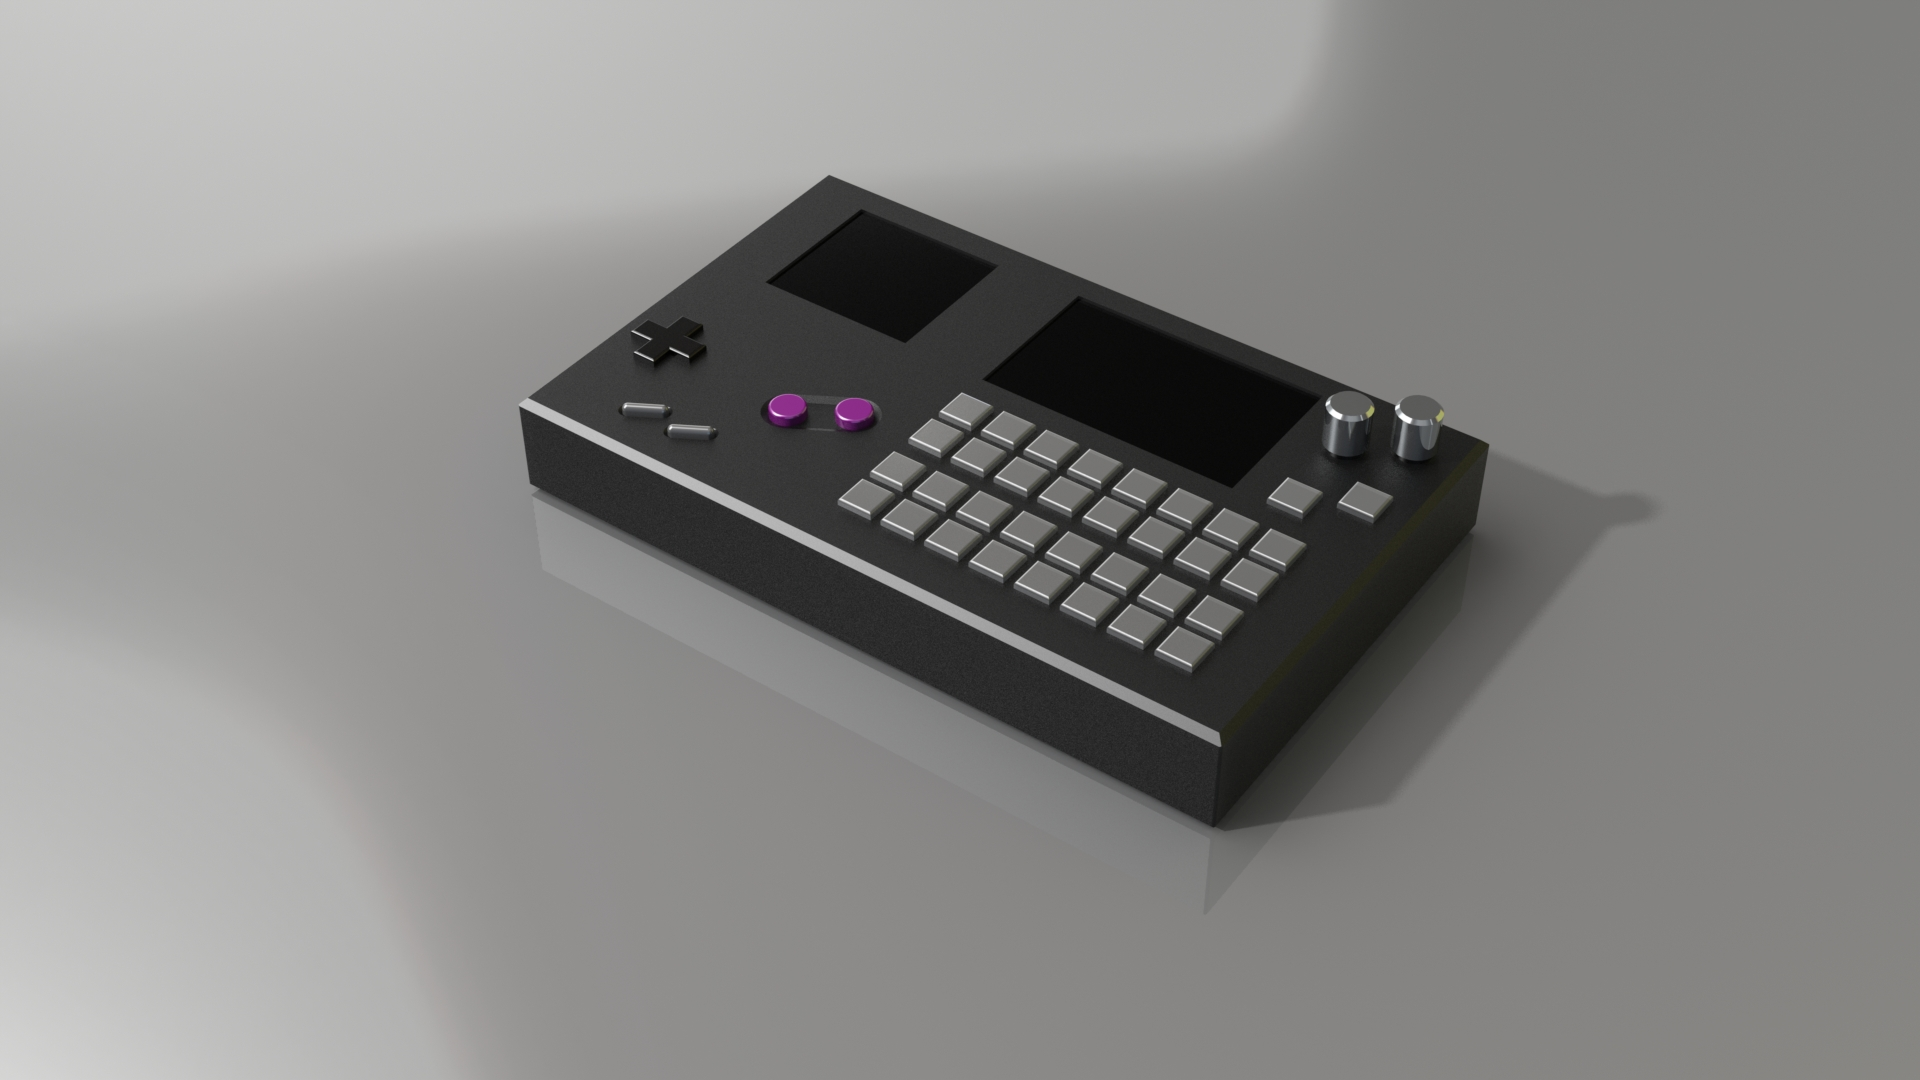
\includegraphics[width=1.1\linewidth]{volca-gb-render.JPG}
            \caption{3D render made with SolidWorks and Photoview 360 to show the concept look of the final product.}
        \end{figure}
    \end{landscape}
 \end{appendices}




\end{document}
